\documentclass[11pt]{beamer}
\usetheme{Singapore}

\usepackage[utf8]{inputenc}
\usepackage[T1]{fontenc}
\usepackage{soul}
\usepackage{graphicx}


\graphicspath{{../Figures/}}

\def\et{{\it et al.}}


\author{Cody Glickman \\ CPBS Update Talk}

\title{Hodgepodge Metagenomics: \\ A collection of novel tools for viral and bacterial sequences}
%\subtitle{}
%\logo{}

\date{ 
\includegraphics[height=2cm, width=2cm]{lablogo.png} \\ Jan 29th, 2018}
%\subject{}
\setbeamercovered{transparent}
\setbeamertemplate{navigation symbols}{}
\setbeamertemplate{theorems}[numbered]

\begin{document}
	\maketitle
	\begin{frame}{Table of Contents}
		\tableofcontents
		%\column{0.4\textwidth}
		%\includegraphics[height=5.5cm, width=5cm]{kaola.png}
		%\end{columns}
	\end{frame}
	
	
%Research UPdate and highlight certain things
% Hawaii soil Asthma
	
\section{Introduction}
\subsection{}

	\begin{frame}{Nontuberculous Mycobacterial (NTM) Infections}
		%Tuberculous!!!
		\begin{block}{Number of Cases}
		The number of NTM cases is estimated over 100K
		\end{block}
		
		\begin{block}{Increasing Case}
		The rate of cases is estimated to grow at 8\% every year
		\end{block}
		
		
		\begin{block}{Populations at risk of developing NTM}
		\begin{itemize}
		\item Immunocompromised individuals 
		\item Patients with lung damage or malfunction 
		\item Residing in warm costal areas especially Hawaii
		\item older and female
		\end{itemize}
		\end{block} 
		
		\begin{block}
		
		\end{block}
		
	\tiny{Strollo SE, et al. Ann Am Thorac Soc. 2015 \\
	Adjemian J, et al. Am J Respir Crit Care Med. 2012}
	
	\end{frame}
	
	\begin{frame}{Understanding Why NTM Develops}
	
	\begin{block}{Hawaiian Soil Project}
	\vspace{0.3cm}
		\begin{columns}
		\column{0.4\textwidth}
		Identifying important soil characteristics for NTM soil culture 
	
		
		
		
		\column{0.5\textwidth}
		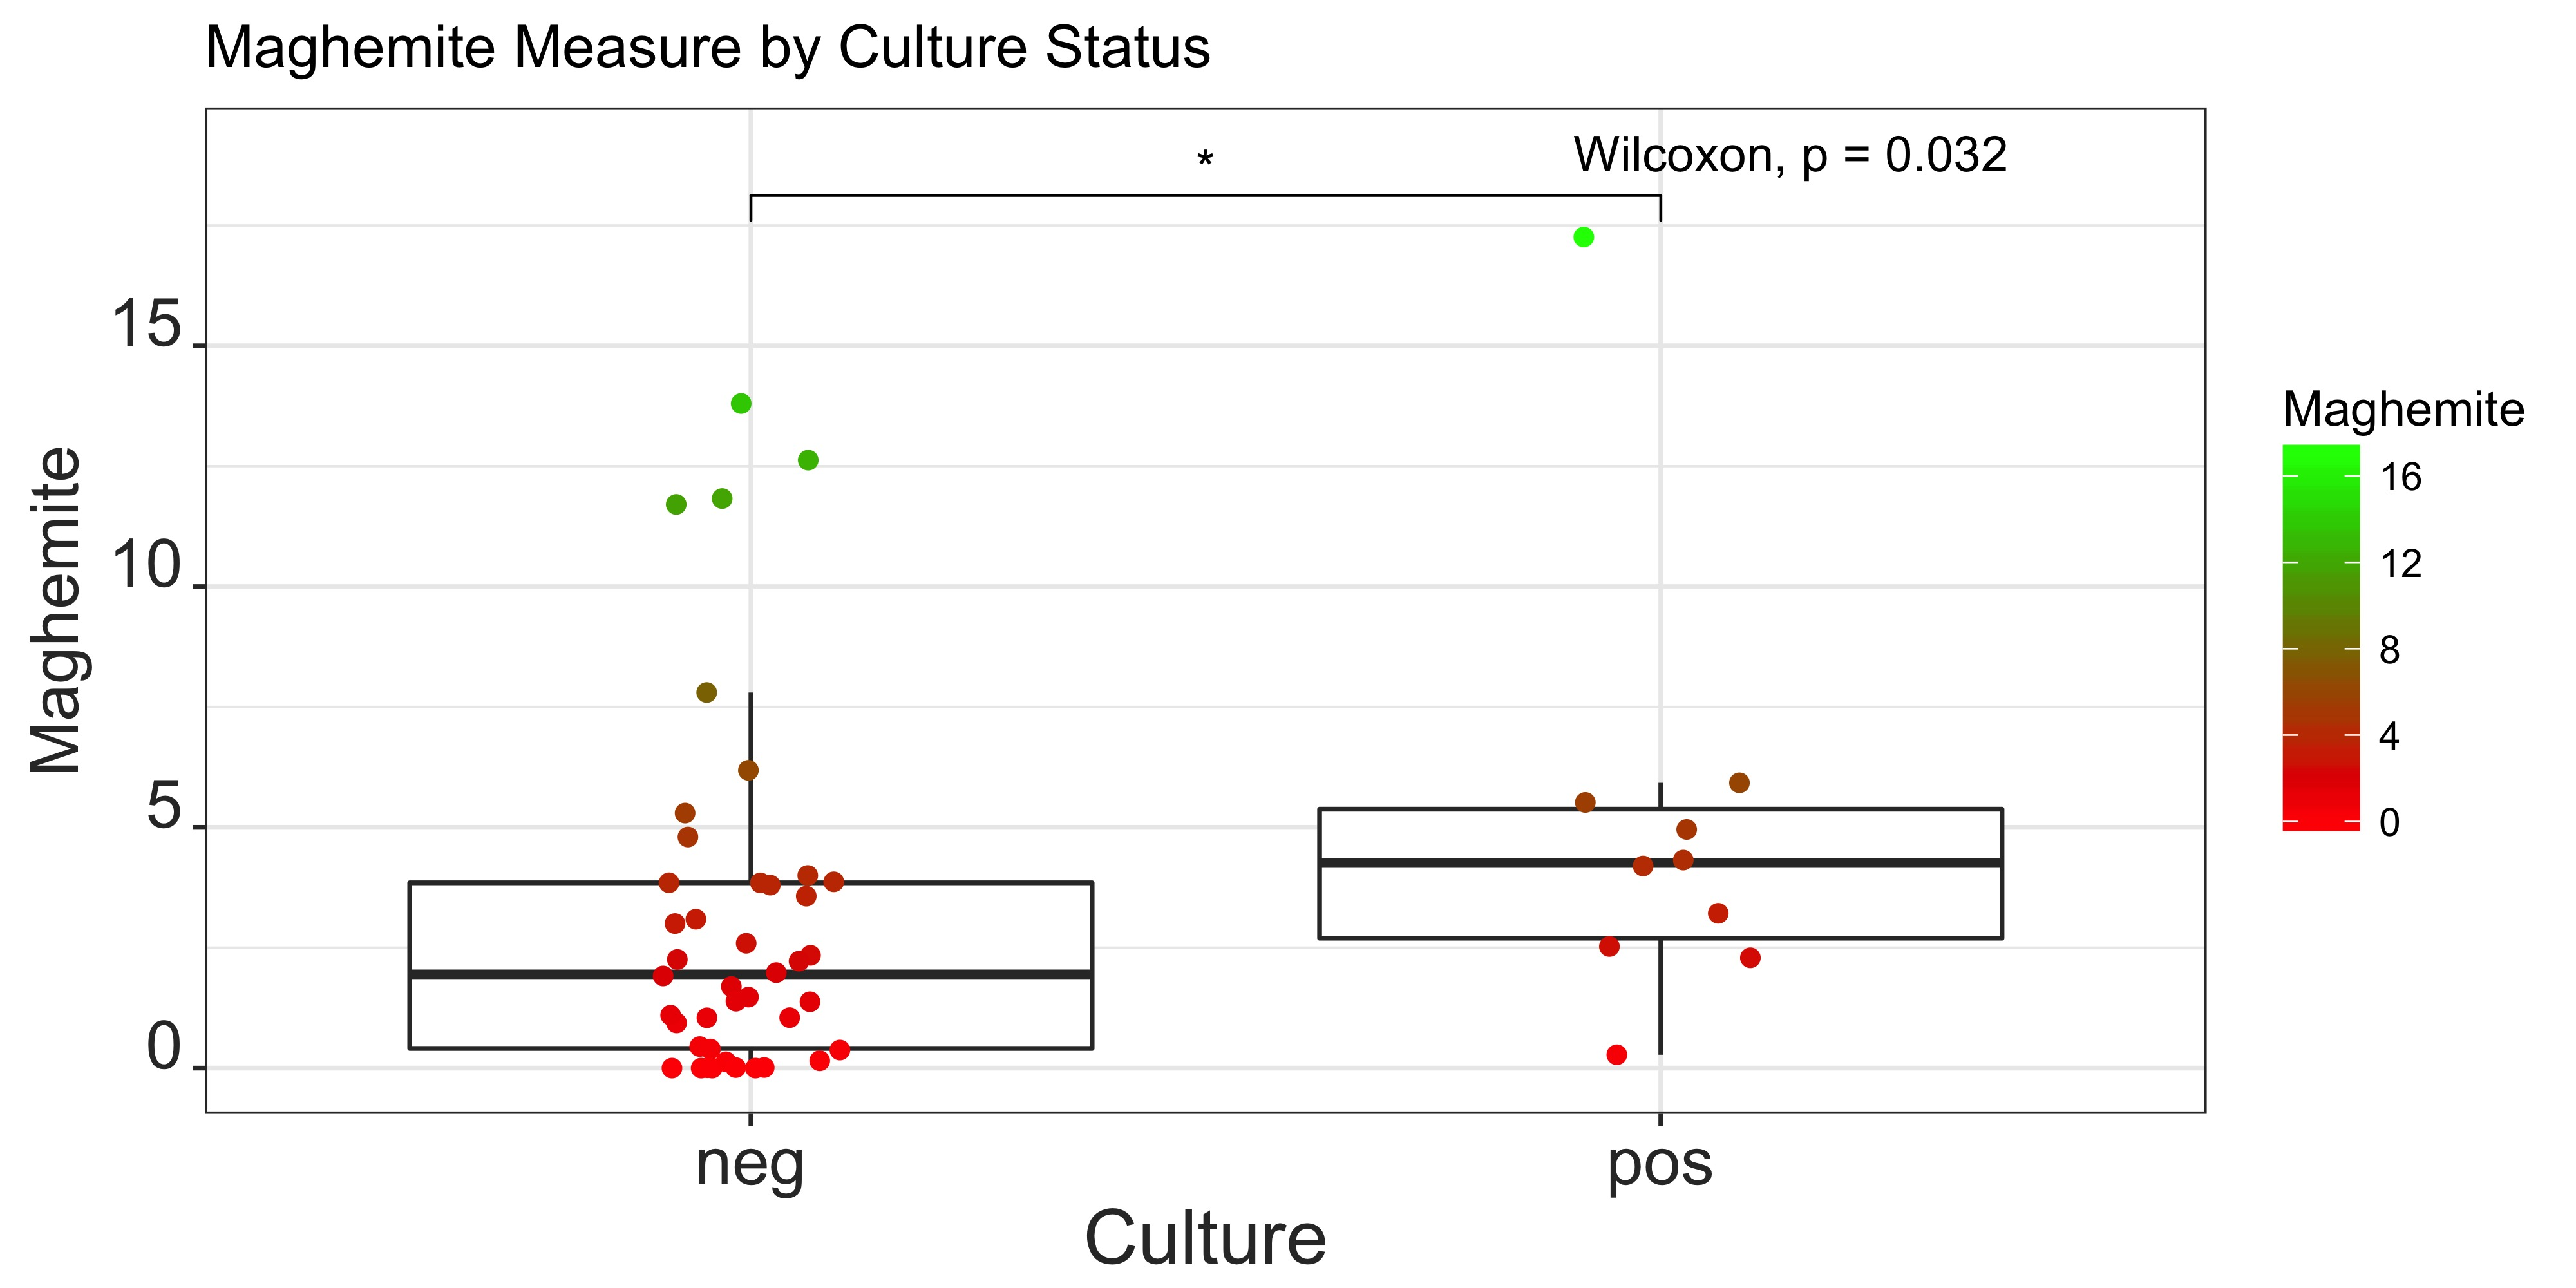
\includegraphics[height=3.5cm, width=5cm]{soil.jpeg}
		\end{columns}
	
	\end{block}
	
	\begin{block}{Pulmonary NTM}
	\begin{itemize}
	\item 90\% of NTM cultures are from respiratory samples
	\item The lung has the lowest abundance of DNA viruses in the human niche
	\end{itemize}
	\end{block}
	
	\vspace{0.3cm}
	
	\tiny{O'Brien, R., et al. American Review of Respiratory Disease 1987 \\ Aziz R., et al. Frontiers in microbiology 2015}

	
	\end{frame}
	
	
	\begin{frame}{Of "Viral" Importance}
	\begin{columns}
	\column{0.7\textwidth}
	
	\begin{block}{Bacteriophages aka Phages}
	Phages are DNA viruses that infect prokaryotes
	\end{block}
	
	\begin{block}{Bacteriophage Adherence to Mucus (BAM)}
	\begin{itemize}
	\item \alert{Phages act as an innate immune system in mucosal tissues}
	\item Prior studies identified Ig-like motifs in induced phages from Pseudomonas cultures
	\end{itemize}
	\end{block}
	
	\begin{block}{Phages in the Lungs}
	The abundance of phages is significantly lower in the lungs
	\end{block}
	
	\column{0.4\textwidth}
	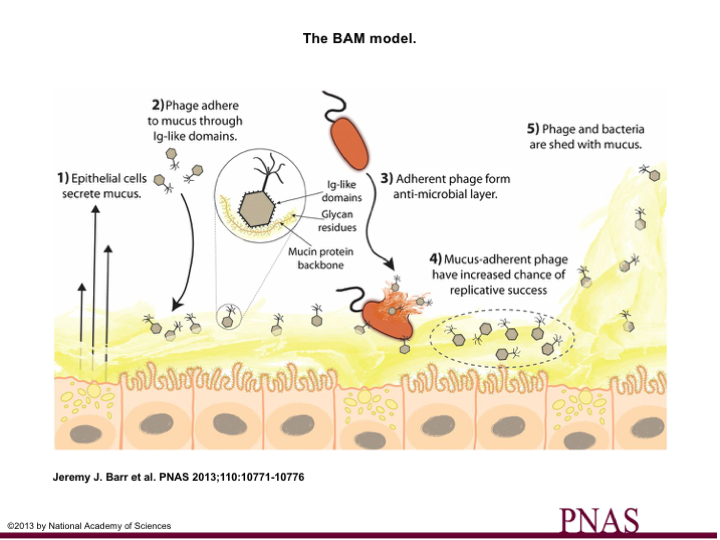
\includegraphics[height=5.5cm, width=5cm]{barr.png}
	\end{columns}

	
	
	
	\end{frame}
	
	
	\begin{frame}{Molecular Methods to Study Phages}
	\begin{columns}
	\column{0.5\textwidth}
	\begin{block}{Difficulties of phage study}
	\begin{itemize}
		\item Lack of universal marker gene
		\item Sequence heterogeneaity 
		\item Misclassification in databases
	\end{itemize}
	\end{block}
		
		
	\begin{block}{Phage Isolation Methods}
	\begin{itemize}
		\item Biological filtration
		\item In Silico Methods
	\end{itemize}
	\end{block}
	
	\column{0.5\textwidth}
	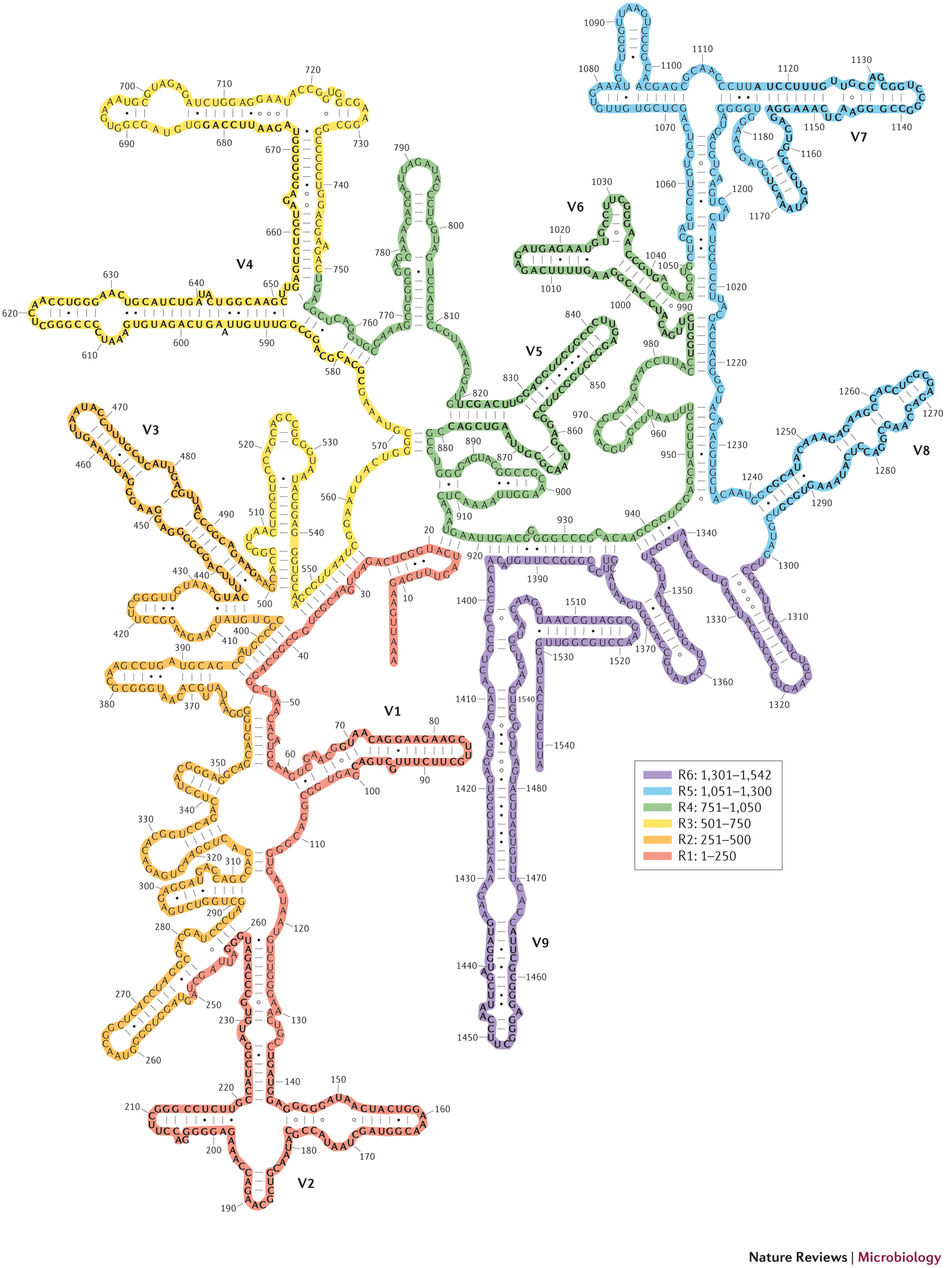
\includegraphics[height=5.5cm, width=5cm]{ribosome.jpg}
	\end{columns}
		
	
	\end{frame}

	
	\begin{frame}{Objective}
	
	Develop new tools and incorporate them into pipelines to identify and quantify bacteriophage elements in shotgun metagenomic sequences.
	
	\begin{block}{Secondary Goal}
	Identify relationships between bacteria and phages using abundance quantification across multiple studies. 
	\end{block}
	\end{frame}


	
\section{Metagenomic Simulation Study}
\subsection{}
	%% Unbiased study of all genetic material 
	\begin{frame}{Metagenomics}
	\begin{columns}
	\column{0.5\textwidth}
	\begin{block}{What is Metagenomics?}
	Unbiased study of all genetic material in a sample
	\end{block}
	\begin{block}{Importance of Metagenomics}
	\begin{itemize}
	\item Functional potential of a sample
	\item Species level distinctions
	\item Due to lack of a universal gene marker, phages are studied by metagenomics
	\end{itemize}
	\end{block}
	
	\column{0.5\textwidth}
	Include Photo Mosaic Here
	%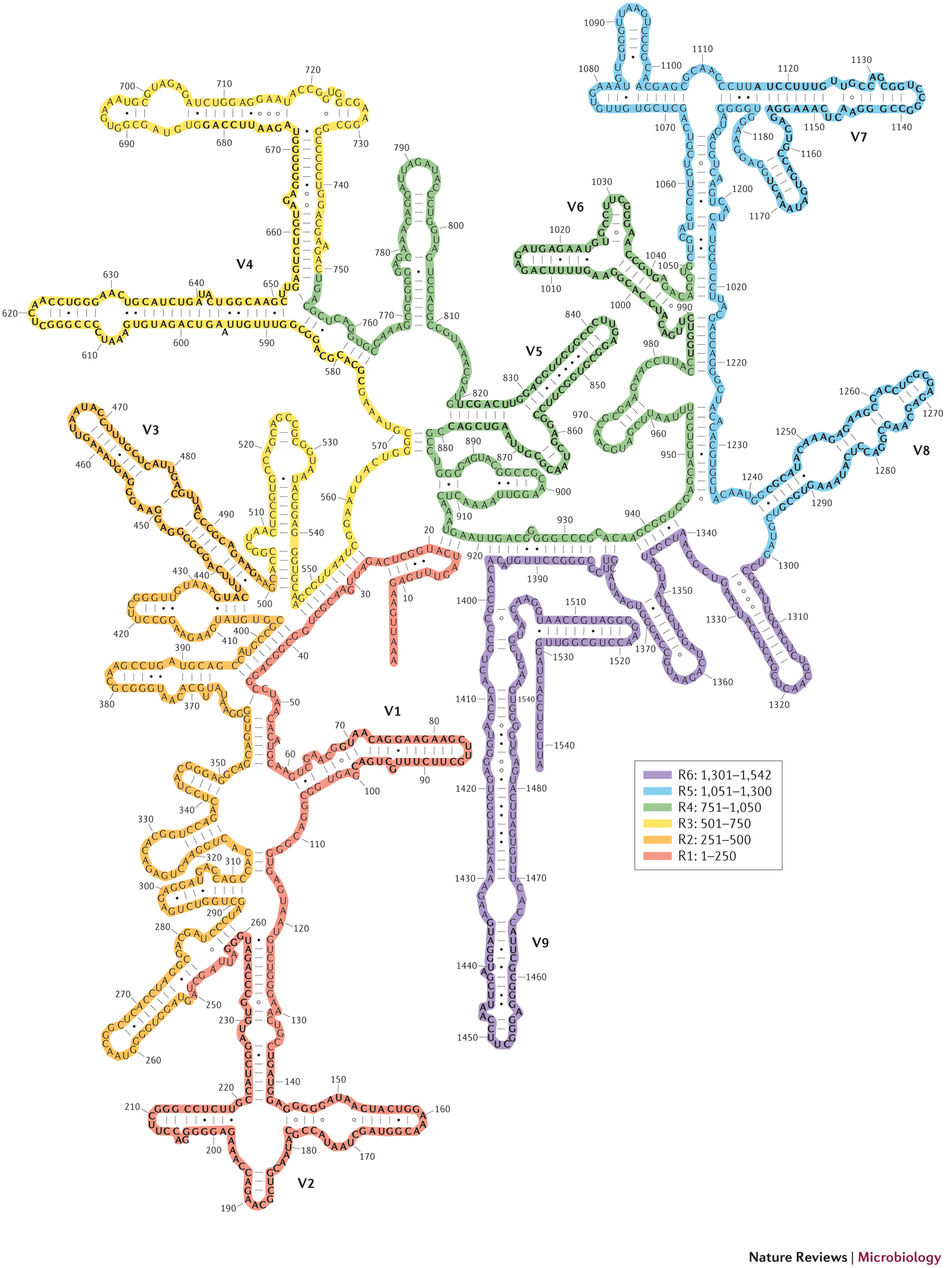
\includegraphics[height=5.5cm, width=5cm]{ribosome.jpg}
	\end{columns}
	\end{frame}
	
	%molecular ecology reasources

	
	\begin{frame}{Metagenomics Gold Standard} 
	\begin{columns}
	\column{0.6\textwidth}
	\begin{block}{Critical Assessment of Metagenome Interpretation (CAMI)}
	\begin{itemize}
	\item 1300 newly sequenced organisms collected in simulated dataset 
	\item 25 programs and 36 biobox implementations (binners, assemblers, taxonomic profilers)
	\end{itemize}
	\end{block}
	
	\begin{block}{Pyrite Standard}
	Viral elements worsened abundance estimates in taxonomic profilers
	\end{block}
	
	\vspace{0.3cm}
	\tiny{Sczyrba, A., et al. Nature Methods 2017}
	
	
	\column{0.5\textwidth}
	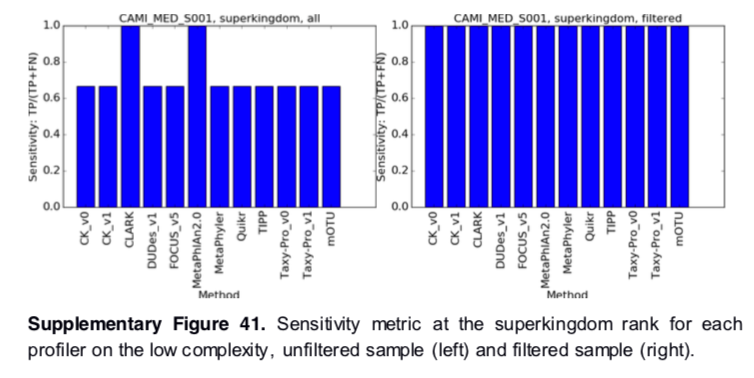
\includegraphics[height=5cm, width=5.5cm]{filtered.png}
	\end{columns}
	
	\end{frame}
	
	
	\begin{frame}{Improving Taxonomic Profiling}
	
	
	\begin{block}{CAMI and Viruses}
	Filtering viruses improves abundance profile estimates for bacteria
	\end{block}
	\vspace{0.1cm}
	\begin{columns}
	\column{0.5\textwidth}
	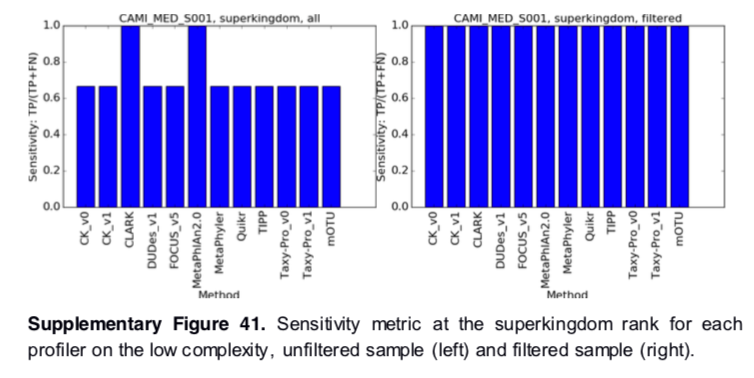
\includegraphics[height=5cm, width=5.5cm]{filtered.png}
	\end{columns}
	
	\end{frame}
	
	\begin{frame}{Viral Filtration Simulation Study}
	\begin{block}{Study Design}
	30 simulated mixed metagenomes are used to compare the viral contiguous sequence (contigs) identification performance of multiple tools
	\end{block}

	\begin{block}{Sequencing Depth of Experiment} 
	Each metagenome is comprised of 10 million reads
	\end{block}
	\begin{block}{Complexity of Metagenomes}
	8 bacteria and 8 phages comprise the low complexity samples in each metagenome
	\end{block}

	\end{frame}
	
	\begin{frame}{Genomes in Simulation}
	\begin{columns}
		\column{.5\textwidth}
			\begin{block}{Virus - 0.12 Mb}
			\begin{itemize}
			\item Bacillus phage Pony
			\item Caulobacter phage CcrColossus
			\item Mycobacterium phage Bxb1
			\item Mycobacterium phage Che9d
			\item Mycobacterium phage TM4
			\item Pseudomonas phage vB-PaeM-C2-10-Ab1
			\item Staphylococcus phage CNPH82
			\item uncultured phage crAssphage
			\end{itemize}
			\end{block}	
		\column{.6\textwidth}
			\begin{block}{Bacteria - 4.72 Mb}
			\begin{itemize}
			\item Bacillus subtilis subs. subtilis 168
			\item Clostridium acetobutylicum ATCC 824
			\item Clostridium perfringes str. 13
			\item Lactococcus lactis subsp. lactis Il1403
			\item Pseudomonas aeruginosa LESB58
			\item Staphylococcus aureus subsp. aureus N315
			\item Streptococcus pyogenes M1 476
			\item Xylella fastidiosa 9a5c
			\end{itemize}
			\end{block}
	\end{columns}
	\end{frame}
	
	\begin{frame}{Tools Used in Study}
	The tools used in this study are selected based on recent publications
	\begin{block}{Assembler}
	MEGAHIT - Effective at assembling viromes \\
	\tiny{Roux, Simon, et al. PeerJ 2017}
	\end{block}
	
	\begin{block}{Filtration Methods}
	VirFinder - Viral contig K-mer identification model \\ 
	\tiny{Ren, Jie, et al. Microbiome 2017}
	
	\large{Blastx - Filtering against a viral protein database} \\
	\tiny{Camacho C., et al. BMC Bioinformatics 2008}
	\end{block}
	
	\end{frame}
	
	\begin{frame}{Tools Used in Study Continued}
	\begin{block}{Simulation Tools}
	BBMAP - a suite of tools designed for sequencing data \\
	\tiny{Bushnell, B., JGI 2016}
	\end{block}
	
	\begin{block}{Taxonomic Identification}
	Kraken - A reference-free K-mer taxonomic identifier \\
	\tiny{Wood, Derrick E., and Steven L. Salzberg Genome 2014}
	
	\large{Blastx - Referenced against a viral protein database} \\
	\tiny{Camacho C., et al. BMC Bioinformatics 2008}
	\end{block}
	
	\begin{block}{Prophage Identification}
	Phaster - A popular prophage discovery web tool  \\
	\tiny{Arndt, David, et al., Nucleic Acids Research 2016}
	\end{block}
	\end{frame}
	
	
	\begin{frame}{Performance Measurements}
	
	\begin{block}{True Viral Contigs}
	True viral contigs are defined by BLAST hits (E-value 10\^-05) against a custom database of reference phages and bacterial prophage elements. 
	\end{block}
	
	\begin{block}{Term Definitions}
	\begin{columns}
	\column{.3\textwidth}
	TP = True Positive
	\column{.3\textwidth}
	FP = False Positive
	\column{.35\textwidth}
	FN = False Negative
	\end{columns}
	
	\end{block}
	\vspace{-0.2cm}
	\begin{block}{Performance Metrics}
	\begin{itemize}
	\item Recall = TP / (TP + FN)
	\item Precision = TP / (TP + FP)
	\item F1 = (2*TP) / (2*TP + FP + FN)
	\end{itemize}
	\end{block}
	\end{frame}
	
	\begin{frame}{Recall}
	\vspace{-1cm}
	\center
	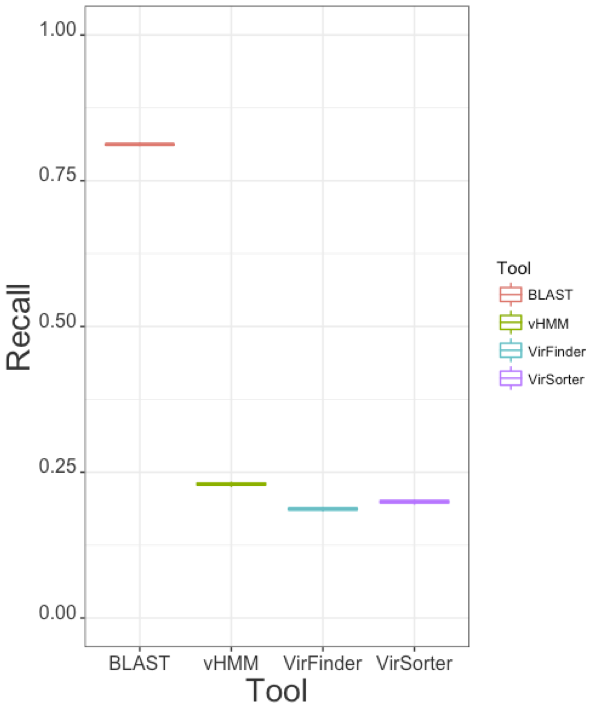
\includegraphics[height=5cm, width=7cm]{Recall.png}
	\end{frame}
	
	\begin{frame}{Precision}
	\vspace{-1cm}
	\center
	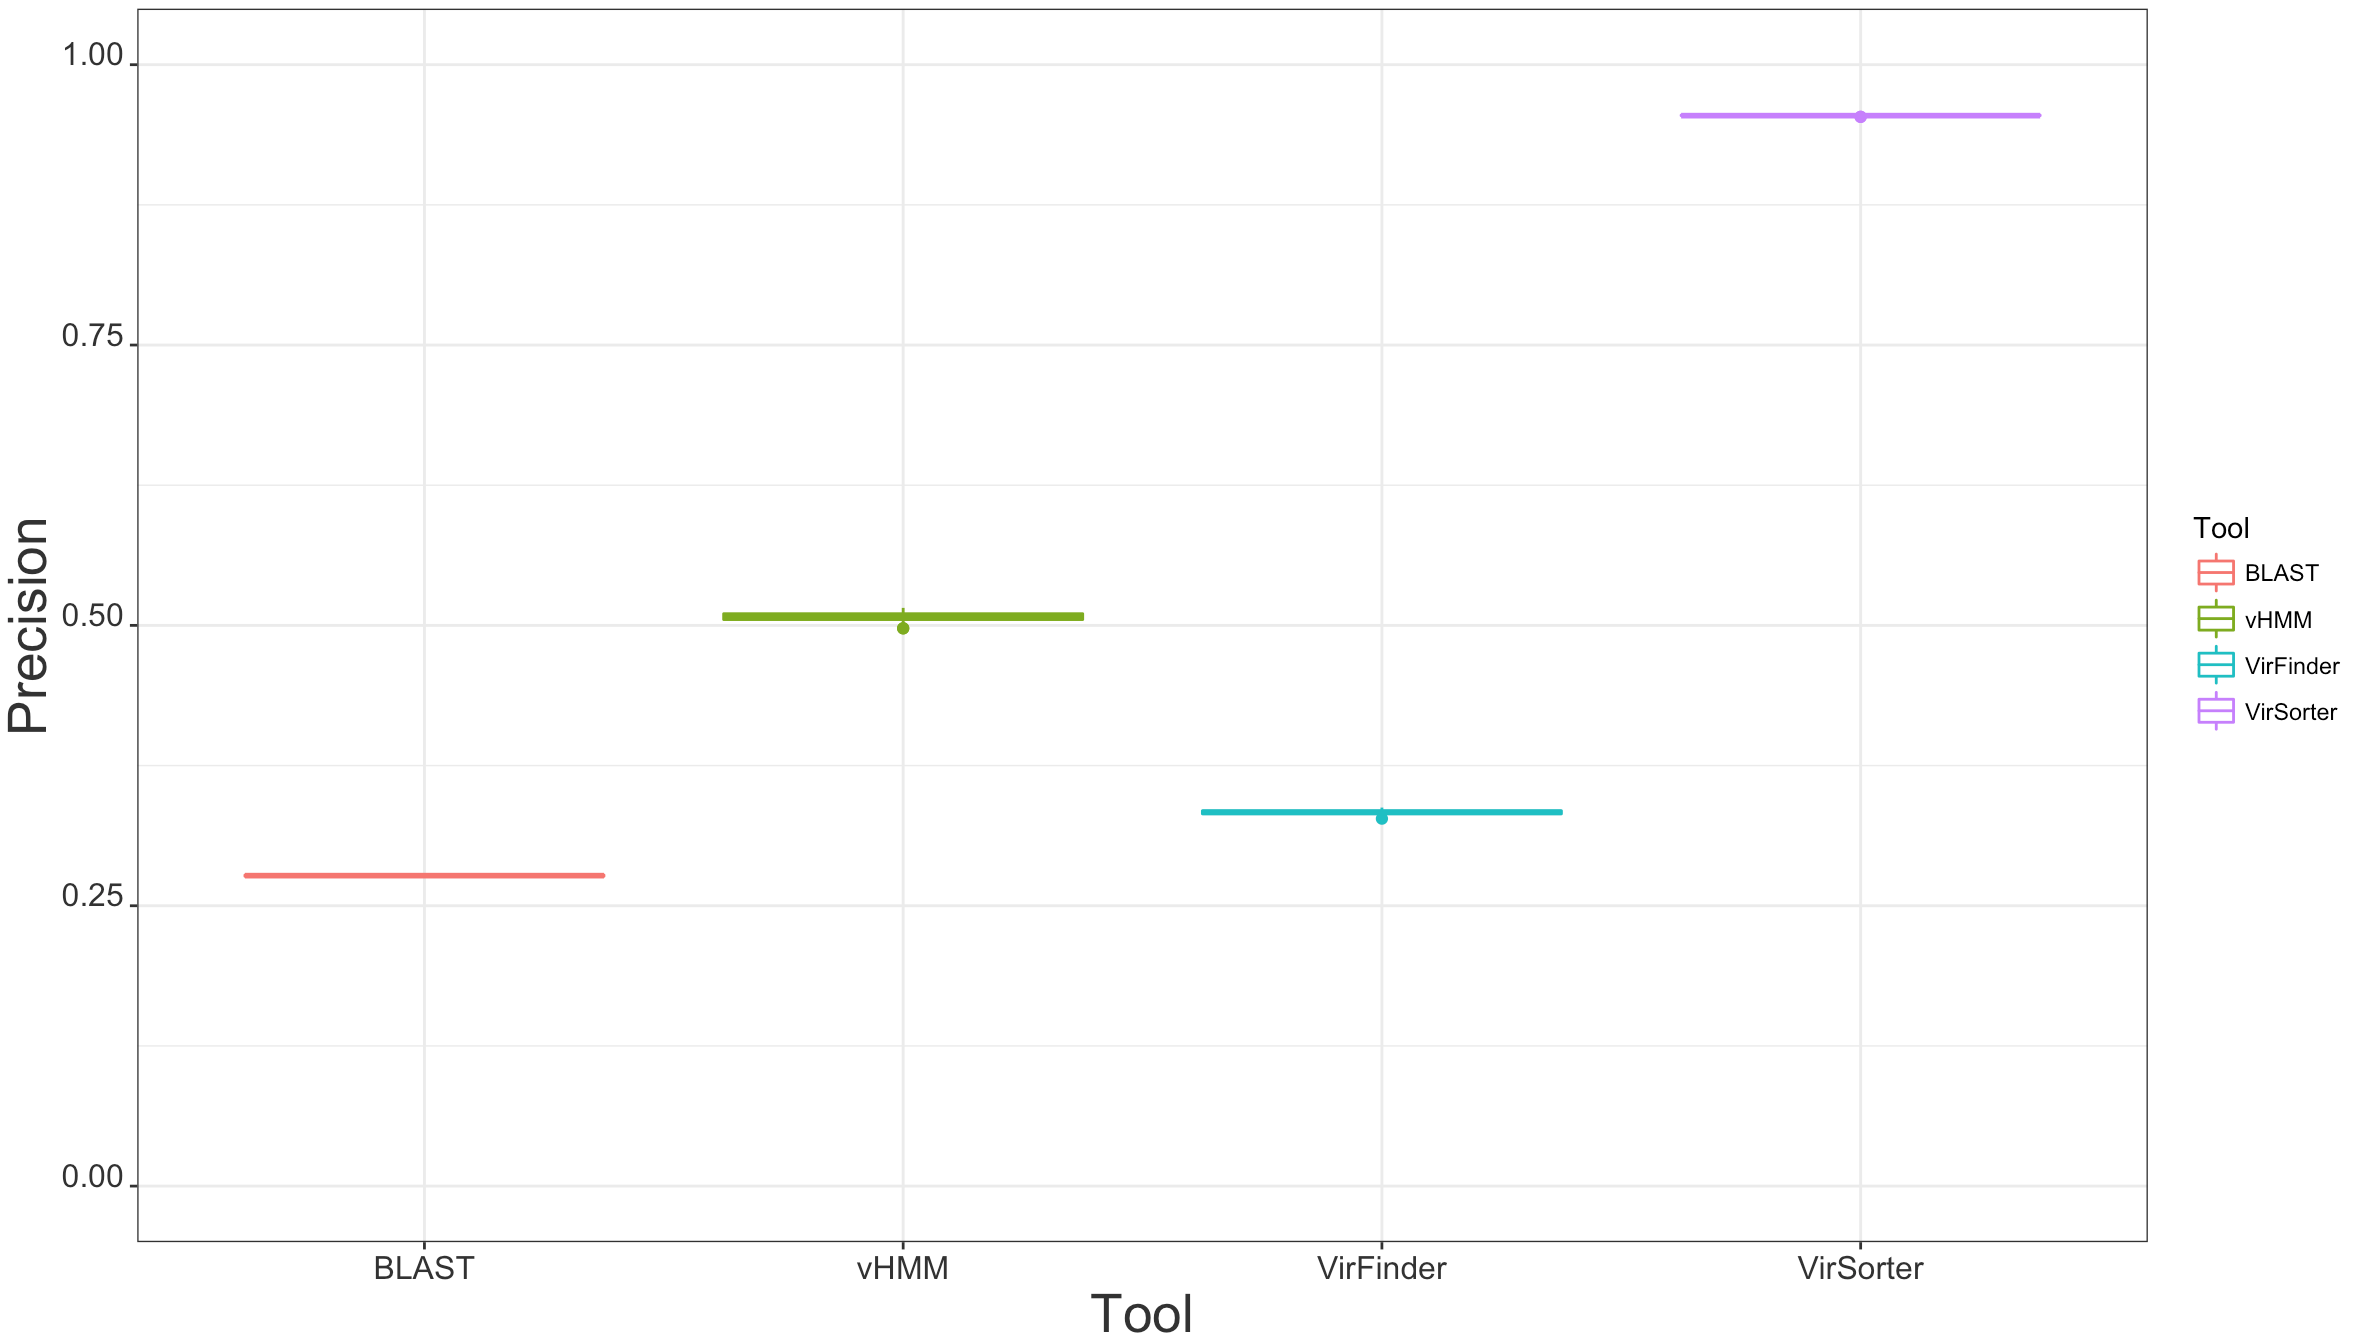
\includegraphics[height=5cm, width=7cm]{Precision.png}
	\end{frame}
	
	\begin{frame}{F1}
	\vspace{-1cm}
	\center
	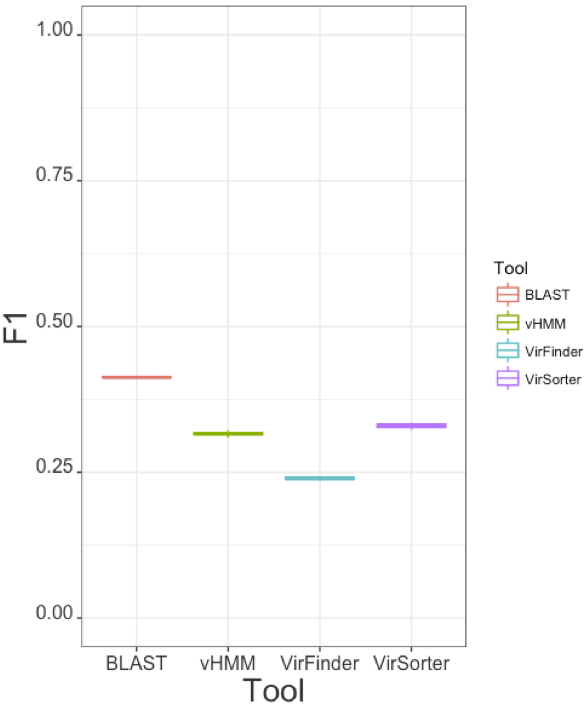
\includegraphics[height=5cm, width=7cm]{F1.png}
	\end{frame}
	
	\begin{frame}{Conclusions and Future Directions}
	
	\begin{block}{Performance}
	The variance of performances suggests that no one tool is optimal for viral filtration
	\end{block}
	
	\begin{block}{Expansion of Tools}
	Inclusion of binners MetaBat and MetaWatt 3.5
	\end{block}
	
	\begin{block}{Expanded Dataset}
	Filter viral elements from CAMI data
	\end{block}
	
	\begin{block}{Tool Parameter Optimization}
	VirFinder is currently trained against only phages 
	\end{block}
	
	\end{frame}
	

\section{GRAB}
\subsection{}

	\begin{frame}{Custom BLAST Databases}
	\begin{block}{Command-line BLAST}
	Released in 2008 to allow users to run BLAST on local machines
	\end{block}
	
	\begin{block}{makeblastdb Function}
	Allows user to create custom BLAST databases from local sequences
	\end{block}
	
	\begin{block}{Sequence Batch Retrieval}
	NCBI Webserver, ESearch function, biomart R package
	\end{block}
	
	\end{frame}
	
	\begin{frame}{Current Batch Retrieval} 
	\vspace{-1cm}
	\center
	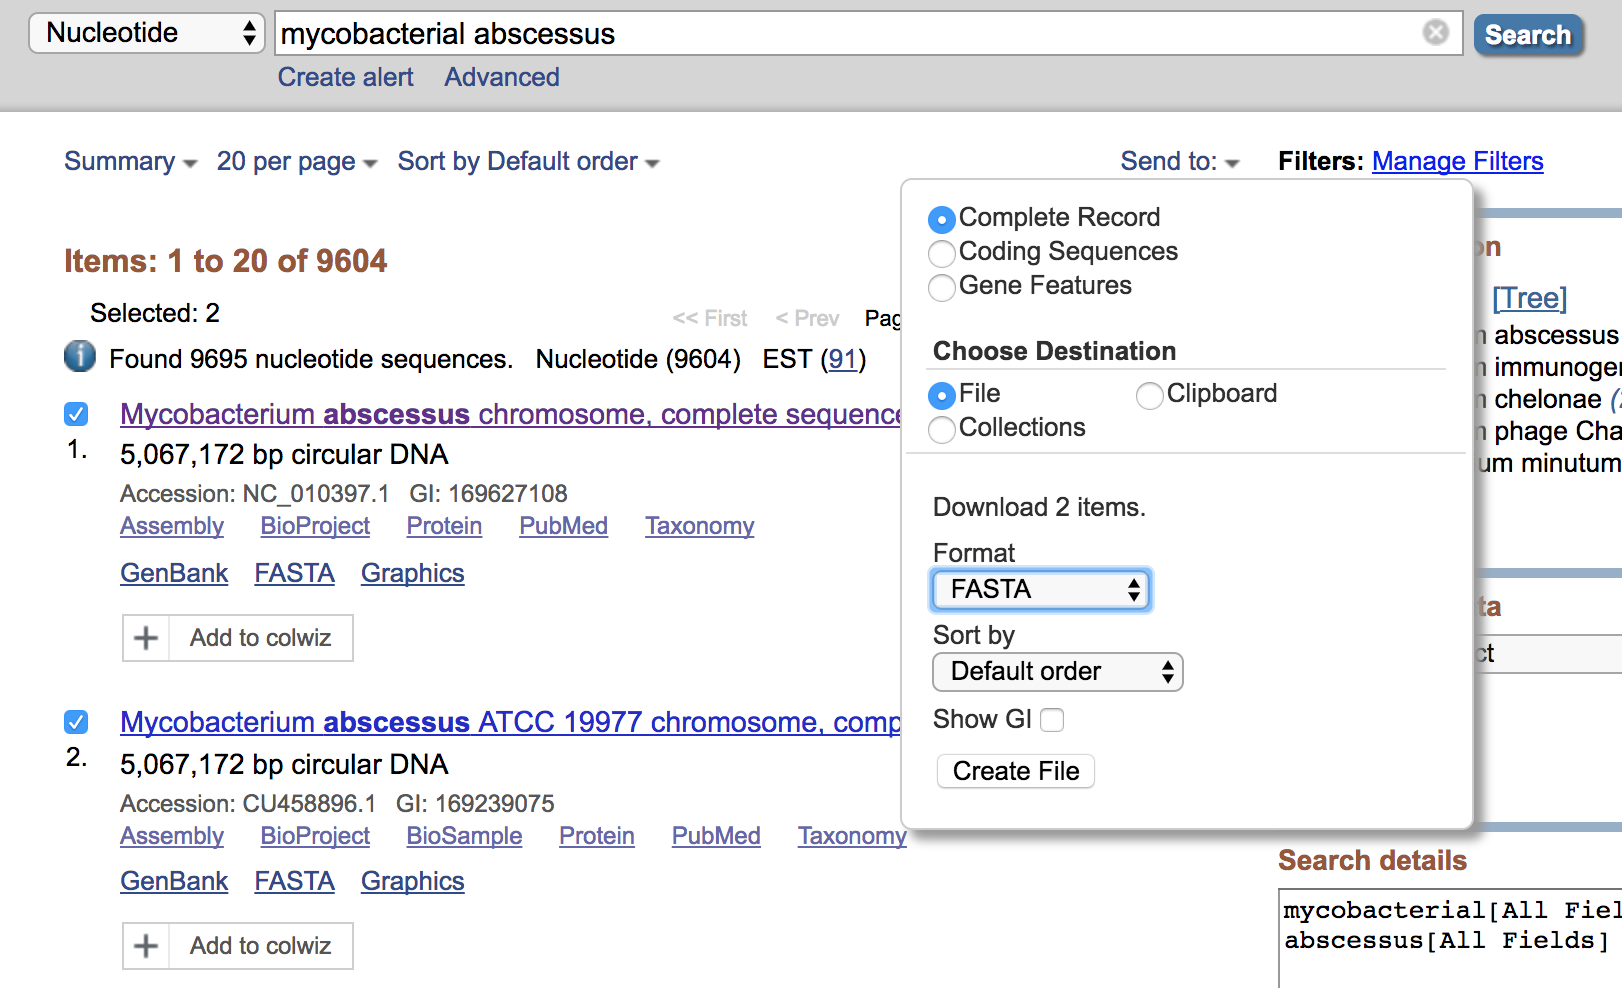
\includegraphics[height=8cm, width=11cm]{Download.png}
	\end{frame}
	
	\begin{frame}{Obstacles to Current Systems}
	\begin{block}{Taxonomic Querying}
	Querying multiple bacteria by taxonomy requires long command \\
	\vspace{0.5cm}
	\tiny{"Mycobacterium abscessus"[Organism] OR "Mycobacterium avium"[Organism]}
	\end{block}
	
	\begin{block}{A Priori Knowledge}
	ESearch requires knowledge of accession numbers to query
	\end{block}
	
	\begin{block}{Required Programming Knowledge}
	The biomart R Package requires knowledge of IDE and data manipulation
	\end{block}
	\end{frame}
	
	\begin{frame}{Genomic Retrieval and Blast Database Creation (GRAB)}
	\begin{block}{A Batch Retrieval System for Biologists}
	Well-Documented Command Line and Web interface
	\end{block}
	
	\begin{block}{Allows for Taxonomic Querying}
	\end{block}
	
	
	
	\end{frame}
	
	

	
	

	

	
	

\section{BUD}
\subsection{}
	

	

	
\section{}
	
	\begin{frame}{}
	\vspace{1cm}
	{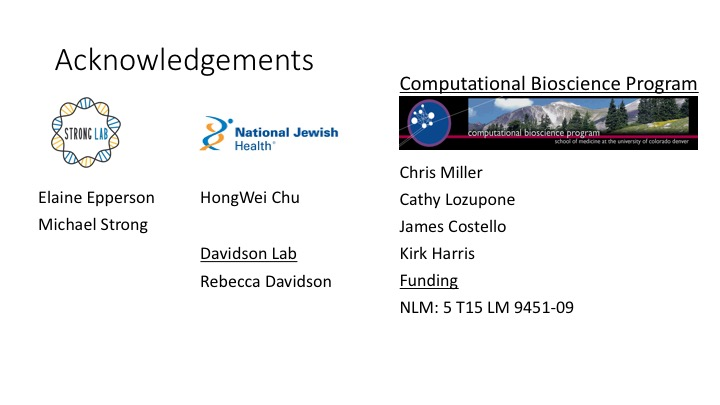
\includegraphics[height=8cm, width=11cm]{Acknowledge.jpg} }
	\end{frame}
	
	
	\begin{frame}{Questions?}
	
	Cody Glickman \\ 
\includegraphics[height=2cm, width=2cm]{lablogo.png} \\ cody.glickman@ucdenver.edu \\ \alert{www.github.com/glickmac} \\ www.codyglickman.com
	\end{frame}
	
	
	\begin{frame}{Bias in Average Fold Coverage by GC}
	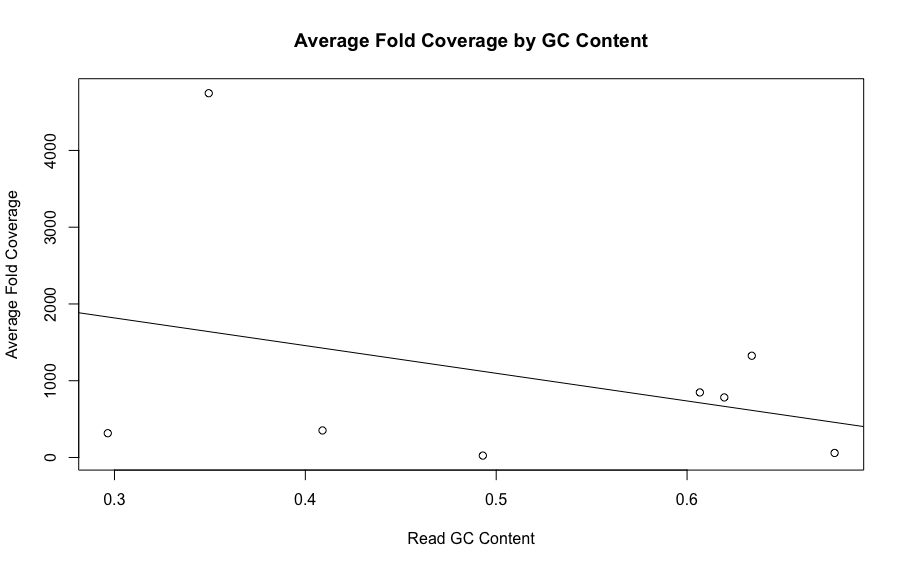
\includegraphics[height=8cm, width=11cm]{Viral_Coverage_by_GC.png}
	\end{frame}
	
	
	\begin{frame}{References}
	\tiny{ Barr, Jeremy, et al., PNAS 2013 \\ Tariq, Mohammad, et al., Frontiers in Microbiology 2015}
	\end{frame}
	
	\begin{frame}{My Pipeline}
	\vspace{-1cm}
	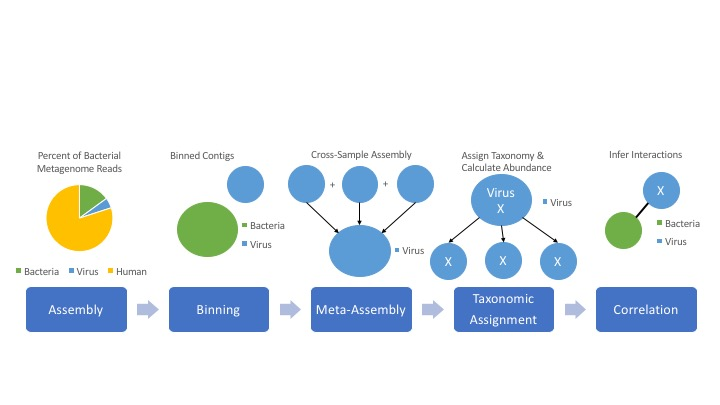
\includegraphics[height=6cm, width=11cm]{figure_2_updated.jpg}
	\end{frame}
	
\end{document}